\documentclass{article}

\title{Lab-6}
\author{2347139}
\date{\today}


\usepackage{listings}
\usepackage{color}
\usepackage{graphicx}

\definecolor{dkgreen}{rgb}{0,0.6,0}
\definecolor{gray}{rgb}{0.5,0.5,0.5}
\definecolor{mauve}{rgb}{0.58,0,0.82}

\lstset{frame=tb,
  language=Java,
  aboveskip=3mm,
  belowskip=3mm,
  showstringspaces=false,
  columns=flexible,
  basicstyle={\small\ttfamily},
  numbers=left,
  numberstyle=\tiny\color{gray},
  keywordstyle=\color{blue},
  commentstyle=\color{dkgreen},
  stringstyle=\color{mauve},
  breaklines=true,
  breakatwhitespace=true,
  tabsize=3
}
\begin{document}
\maketitle
\begin{lstlisting}
    interface Build<build> {
        public void showBotDetails();
    
        public void createGuild(String guildName);
    
        public void getBotPermission(int permission);
    
        public void showBotDetails(String clientName);
    
    }
    
    interface Command<Cmd> {
        public void getMembers();
    
        public void slashCommand(String user);
    }
    
    class Builder implements Build<Integer> {
        public String botName;
        protected String discordToken;
    
        Builder(String botName, String discordToken) {
            if (discordToken.isEmpty()) {
                System.out.println("Token not found");
            }
            this.botName = botName;
            this.discordToken = discordToken;
        }
    
        public void showBotDetails() {
            System.out.println("Discord Bot with " + botName + " created in your account");
    
        }
    
        public void createGuild(String guildName) {
            System.out.println("Created a guild " + guildName + " associated to the bot");
        }
    
        public void getBotPermission(int permission) {
            boolean isAdmin = true;
            boolean isMod = true;
            boolean BAN_MEMBERS = true;
            boolean KICK_MEMBERS = true;
            if (permission == 0) {
                System.out.println("The Bot created has 0 permission");
            }
            if (isAdmin && isMod && BAN_MEMBERS && KICK_MEMBERS) {
                System.out.println("The Bot is set full permission");
            }
    
        }
    
        public void showBotDetails(String clientName) {
            System.out.println("Discord Bot with " + botName + " created for client" + clientName);
        }
    
    }
    
    class SlashCommands implements Command<String> {
    
        String botName;
        String discordName;
    
        SlashCommands(String botName, String discordName) {
            this.botName = botName;
            this.discordName = discordName;
        }
    
        public void getMembers() {
            System.out.println("Getting members of the text channel");
            System.out.println("Channel members are : Elumeveguy\n" + //
                    "Emojorekes\n" + //
                    "Eroxihisom\n" + //
                    "Ulelabutuk\n" + //
                    "Ayibiciqeb\n" + //
                    "Oguyocuxas\n" + //
                    "Uxibabujen\n" + //
                    "Epiwimaguk\n" + //
                    "Idenefibiy\n" + //
                    "Amarebamat");
    
        }
    
        public void slashCommand(String user) {
            // String command='ban';
            System.out.println("Ban User ");
            System.out.println("user " + user + " is banned");
    
        }
    
    }
    
    class Generic {
    
        public static void main(String[] args) {
            Builder b1 = new Builder("john doe Bot", "sjdksnsm29327323");
            b1.showBotDetails();
            b1.createGuild("Main Guild");
            b1.getBotPermission(1);
            b1.showBotDetails();
            SlashCommands command = new SlashCommands("bob bot", "bob's server");
            command.getMembers();
            command.slashCommand("someone");
        }
    
    }
\end{lstlisting}

\section*{Output}
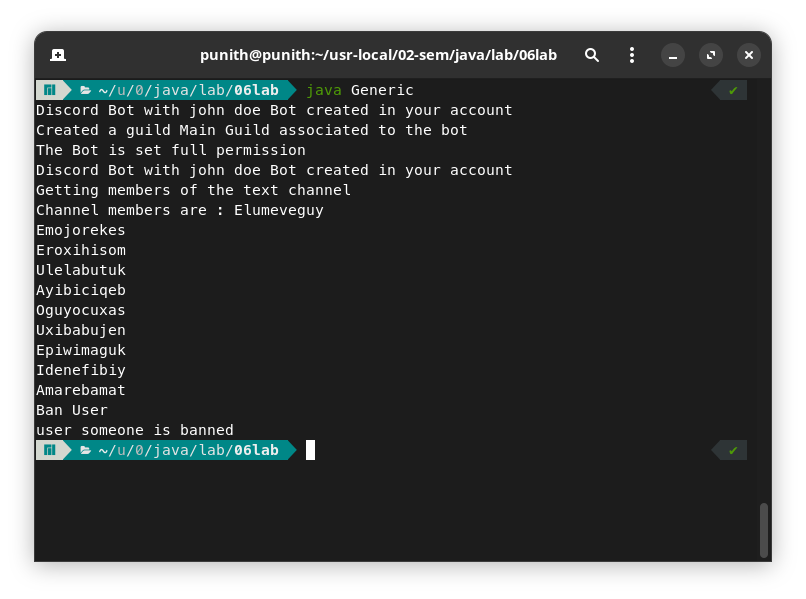
\includegraphics[width=11cm, height=9cm]{./images/01.png}

\end{document}
